\documentclass{standalone}


\usepackage{tikz}
\usetikzlibrary{arrows}

\begin{document}
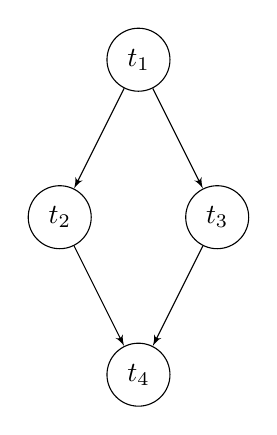
\begin{tikzpicture}[auto, node distance=2cm,>=latex']
\node[circle,draw,minimum size=.8cm] (t1) {$t_1$};
\node[circle,draw,minimum size=.8cm,below of = t1,xshift=-1cm] (t2) {$t_2$};
\node[circle,draw,minimum size=.8cm,below of = t1,xshift=1cm] (t3) {$t_3$};
\node[circle,draw,minimum size=.8cm,below of = t2,xshift=1cm] (t4) {$t_4$};

\draw [->] (t1) -- (t2);
\draw [->] (t1) -- (t3);
\draw [->] (t2) -- (t4);
\draw [->] (t3) -- (t4);
    
\end{tikzpicture}

\end{document}